\documentclass[12pt]{article}
\usepackage[spanish]{babel}
\usepackage[utf8]{inputenc}
\usepackage{dirtytalk}
\usepackage{mathrsfs}
\usepackage{blindtext}
\usepackage{csquotes}
\usepackage{mathtools} 	
\usepackage{polynom}
\usepackage{amsthm}
 \usepackage{natbib}
\usepackage[margin=1.8cm ]{geometry}
\usepackage{url}
\usepackage{amssymb,amsmath,graphics}
\title{\textbf{Grupos y anillos - Tarea Ciclos ejercicios interesantes}}
\author{
}
\date{\today}
\renewcommand\qedsymbol{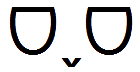
\includegraphics[height=2ex]{Demo_face-removebg-preview.png}}
\begin{document}
\maketitle
\begin{enumerate}
    \item Escribir la siguiente permutación usando notación cíclica:
    $$\begin{matrix}
    1 & 2 & 3 & 4 & 5 & 6 & 7 & 8 & 9\\
    \downarrow & \downarrow & \downarrow & \downarrow & \downarrow & \downarrow & \downarrow & \downarrow & \downarrow \\
    3 & 5 & 7 & 8 & 4 & 6 & 1 & 2 & 9
    \end{matrix}$$
    \begin{proof}[\textbf{Solución:}]
    Llamemos $f$ la permutación presentada en el enunciado ($f\in S_9$). Para hacer uso de la notación cíclica tenemos que observar cuales son los ciclos que realizan los elementos de la permutación, estos ciclos son:
    \begin{align*}
        &1\to3\to7\to1\\
        &2\to5\to4\to8\to2\\
        &6\to6\\
        &9\to9
    \end{align*}
    Luego dado esto la representación cíclica de la permutación $f$ es:
    $$f=(137)(2548)(6)(9)=(137)(2548)$$
    \end{proof}
    \item Sean $\sigma=(123)(456)(78)$ y $\tau=(1357)(26)(4)(8)$ permutaciones (en notación cíclica) de $\{1,2,3,4,5,6,7,8\}$. Escriba en notación cíclica $\sigma\tau, \tau\sigma, \sigma^2, \sigma^{-1}$ y $\tau^{-1}$.
    \begin{proof}[\textbf{Solución: }] Para resolver el ejercicio utilizaremos la notación de arreglo, entonces tenemos que:
    $$\sigma=\begin{pmatrix}
    1 & 2 & 3 & 4 & 5 & 6 & 7 & 8\\
    2 & 3 & 1 & 5 & 6 & 4 & 8 & 7
    \end{pmatrix}$$
    $$\tau=\begin{pmatrix}
     1 & 2 & 3 & 4 & 5 & 6 & 7 & 8\\
     3 & 6 & 5 & 4 & 7 & 2 & 1 & 8
    \end{pmatrix}$$
    Con esto es mucho mas sencillo darnos cuenta de el camino que recorre cada elemento (recordemos que la operación es la composición así que siempre actuamos de derecha a izquierda).
    \begin{itemize}
        \item $\sigma\tau$. El camino que sigue cada elemento es el siguiente:
        $$\begin{matrix}
              &\tau& &\sigma& \\
            1 &\to &3&\to   &1\\
            2 &\to &6&\to   &4\\
            3 &\to &5&\to   &6\\
            4 &\to &4&\to   &5\\
            5 &\to &7&\to   &8\\
            6 &\to &2&\to   &3\\
            7 &\to &1&\to   &2\\
            8 &\to &8&\to   &7\\
        \end{matrix}$$
        De esta forma tenemos que:
        $$\sigma\tau=\begin{pmatrix}
         1 & 2 & 3 & 4 & 5 & 6 & 7 & 8\\ 
         1 & 4 & 6 & 5 & 8 & 3 & 2 & 7
        \end{pmatrix}$$
        Luego los ciclos son:
        \begin{align*}
            &1\to1\\
            &2\to4\to5\to8\to7\to2\\
            &3\to6\to3
        \end{align*}
        Luego la notación cíclica es:
        $$\sigma\tau=(1)(24587)(36)=(24587)(36)$$
        \item $\tau\sigma$. Nuevamente observemos el camino que sigue cada elemento:
        $$\begin{matrix}
              &\sigma& &\tau& \\
            1 &\to &2&\to   &6\\
            2 &\to &3&\to   &5\\
            3 &\to &1&\to   &3\\
            4 &\to &5&\to   &7\\
            5 &\to &6&\to   &2\\
            6 &\to &4&\to   &4\\
            7 &\to &8&\to   &8\\
            8 &\to &7&\to   &1\\
        \end{matrix}$$
        De esta forma tenemos que: $$
        \tau\sigma=\begin{pmatrix}
         1 & 2 & 3 & 4 & 5 & 6 & 7 & 8\\
         6 & 5 & 3 & 7 & 2 & 4 & 8 & 1 \\
        \end{pmatrix}$$
        y los ciclos son:
        \begin{align*}
            &1\to6\to4\to7\to8\to1\\
            &2\to5\to2\\
            &3\to3
        \end{align*}
        Luego la notación cíclica es:
        $$\tau\sigma=(16478)(25)(3)=(16478)(25)$$
        \item $\sigma^2$. El camino de cada elemento es el siguiente:
        $$\begin{matrix}
              &\sigma& &\sigma& \\
            1 &\to &2&\to   &3\\
            2 &\to &3&\to   &1\\
            3 &\to &1&\to   &2\\
            4 &\to &5&\to   &6\\
            5 &\to &6&\to   &4\\
            6 &\to &4&\to   &5\\
            7 &\to &8&\to   &7\\
            8 &\to &7&\to   &8\\
        \end{matrix}$$
        De esta forma tenemos que:
        $$
        \sigma^2=\begin{pmatrix}
         1 & 2 & 3 & 4 & 5 & 6 & 7 & 8\\
         3 & 1 & 2 & 6 & 4 & 5 & 7 & 8 \\
        \end{pmatrix}$$

       Y los ciclos son:

       \begin{align*}
           &1\to3\to2\to1\\
           &4\to6\to5\to4\\
           &7\to7\\
           &8\to8\\
       \end{align*}

       Entonces la notación cíclica es:

       $$\sigma^2=(132)(465)(7)(8)=(132)(465)$$

       \item $\sigma^{-1}$. Recordemos que $\sigma\sigma^{-1}=Id$ entonces el camino es el siguiente:
       $$\begin{matrix}
              &\sigma& &\sigma^{-1}& \\
            1 &\to &2&\to   &1\\
            2 &\to &3&\to   &2\\
            3 &\to &1&\to   &3\\
            4 &\to &5&\to   &4\\
            5 &\to &6&\to   &5\\
            6 &\to &4&\to   &6\\
            7 &\to &8&\to   &7\\
            8 &\to &7&\to   &8\\
        \end{matrix}$$

        De esto podemos ver que que:
        $$
        \sigma^{-1}=\begin{pmatrix}
         1 & 2 & 3 & 4 & 5 & 6 & 7 & 8\\
         3 & 1 & 2 & 6 & 4 & 5 & 8 & 7 \\
        \end{pmatrix}$$

    Y los ciclos son:

    \begin{align*}
        &1\to3\to2\to1\\
        &4\to6\to5\to4\\
        &7\to8\to7\\
    \end{align*}

    Luego en notación cíclica es:
    $$\sigma^{-1}=(132)(465)(78)=(321)(654)(87)$$

    Note que al hacer la representación cíclica del inverso de una permutación podemos decir que el orden de los elementos de cada ciclo se invierte.

    \item $\tau^{-1}$. Por lo que notamos en el anterior ítem, como $\tau=(1357)(26)(4)(8)$ entonces tenemos que:

    $$\tau^{-1}=(7531)(62)(4)(8)=(7531)(62)$$ 
    \end{itemize}
    \end{proof}

    \item Muestre que existen solo tres elementos en $S_4$ que tienen $2$ ciclos de longitud $2$ disjuntos. 
    \begin{proof}[\textbf{Solución: }] Sea $\sigma$ una permutación que solo tiene $2$ ciclos de longitud $2$ disjuntos, es decir es de tipo $[2^2]$, entonces es de la siguiente forma:
    $$\sigma=(\square\text{ }\square)(\square\text{ }\square)$$
    Primero notemos que en esos cuadrados tenemos que organizar los elementos de $\{1,2,3,4\}$ de tal forma que no se repitan entre los ciclos ya que son disjuntos, entonces hay $4!$ maneras de hacerlo.\\
    Ahora notemos que si asumimos esto estaríamos contando casos mas de una vez ya que por ejemplo:
    $$(43)(21)=(34)(12)$$
    Si bien estas dos son distintas en orden de organización de elementos ya que la lista $4321$ es diferente a $3412$ como permutación representa lo mismo, entonces note que en cada ciclo se puede escribir de dos maneras distintas entonces debemos dividir la cantidad previa por:
    $$2\cdot2=2^2=4$$
    Por ultimo observe el siguiente ejemplo:
    $$(43)(21)=(21)(43)$$
    Si bien estas dos permutaciones son la misma como listas no lo son entonces tenemos que tener otro factor en cuenta, que los ciclos como son disjuntos conmutan entre si entonces hay $2!=2$ formas de organizarlos y también debemos dividir la cantidad inicial por esta.\\
    \hfill
    Así concluimos que la cantidad de permutaciones en $S_4$ del tipo $[2^2]$ es:
    $$\frac{4!}{2^2\cdot2!}=\frac{4\cdot3\cdot2\cdot1}{4\cdot2}=3$$
    Particularmente son las siguientes:
    $$\begin{matrix}
        &(12)(34)&
        &(13)(24)&
        &(14)(23)&
    \end{matrix}$$
    \end{proof}

    \item ¿Cuáles son todas las permutaciones de $S_4$ de orden 2?
    \begin{proof}[\textbf{Solución: }] Recordemos que toda permutación puede ser escrita como producto de ciclos disjuntos, además la permutación es de orden 2 si el mínimo común múltiplo de el orden de los ciclos que la componen es de orden 2, eso quiere decir que dada $\sigma\in S_4$ tiene a lo mas ciclos de orden 2, entonces notamos que los dos tipos de permutaciones de este orden son del tipo $[1^22]$ y $[2^2]$, como en el anterior ejercicio ya determinamos las del tipo $[2^2]$ falta determinar cuantas y cuales son del tipo $[1^22]$. Haciendo uso del análisis hecho en el punto anterior se puede concluir que la cantidad de permutaciones de este tipo son:
    $$\frac{4!}{2\cdot2!}=\frac{4!}{4}=3!=6$$
    Luego hay 9 permutaciones de orden 2 en $S_4$ las cuales son:
    $$\begin{matrix}
        &(1)(2)(34)&
        &(2)(3)(14)&
        &(12)(34)&
        \\
        &(1)(3)(24)&
        &(2)(4)(13)&
         &(13)(24)&
        \\
        &(1)(4)(23)&
        &(3)(4)(12)&
        &(14)(23)
    \end{matrix}$$  
    \end{proof}
    \item Escribir los siguientes elementos de $S_8$ como producto de trasposiciones, y encuentre el signo de cada uno:
    $$\begin{matrix}
        \alpha=(1357)(2468)&&\beta=(127)(356)(48)&&\gamma=(135)(678)(2)(4)
    \end{matrix}$$
    \begin{proof}[\textbf{Solución: }] Primero como todas la permutaciones son un producto de ciclos disjuntos podemos realizar su descomposición en trasposiciones de la siguiente manera:
    $$\begin{matrix}
        \alpha=\underbrace{(17)(15)(13)(28)(26)(24)}_{6\text{ }trasposiciones}& &\beta=\underbrace{(17)(12)(36)(35)(48)}_{5\text{ }trasposiciones}& &\gamma=\underbrace{(15)(13)(68)(67)(24)(24)}_{6\text{ }trasposiciones}
    \end{matrix}$$
    Entonces $\alpha,\gamma$ tienen un numero par de trasposiciones y $\beta$ un numero impar de transposiciones, luego por la definición del signo tenemos que:
    $$\begin{matrix}
        \text{sgn}(\alpha)=1&&\text{sgn}(\beta)=-1&&\text{sgn}(\gamma)=1
    \end{matrix}$$
    \end{proof}
    \item Probar que sgn$(\pi\sigma\pi^{-1})=$sgn$(\sigma)$, para todo $\pi,\sigma\in S_n$.\\
    Para este ejercicio presentaremos dos pruebas usando hechos distintos.
    \begin{proof}[\textbf{Demostración 1: }] Dados $\sigma,\pi\in S_n$ Supongamos que $\sigma$ es un producto de $k$ trasposiciones y $\pi$ un producto de $j$ trasposiciones.\\
    Primero observemos que $\pi^{-1}$ también tiene $j$ trasposiciones ya que si $\pi=\tau_1\tau_2\dots\tau_j$, donde cada $\tau_i$ es una trasposición, entonces $\pi^{-1}=(\tau_1\tau_2\dots\tau_j)^{-1}=\tau_j^{-1}\dots\tau_2^{-1}\tau_1^{-1}=\tau_j\dots\tau_2\tau_1$. Luego la cantidad de trasposiciones de $\pi\sigma\pi^{-1}$ es $j+k+j=2j+k$.\\
    Notemos que basta con considerar casos para $\sigma$ y no para $\pi$, ya que independientemente de si es par o impar la paridad de $\pi\sigma\pi^{-1}$ la altera $\sigma$. Si $\sigma$ tiene una cantidad par de trasposiciones, $2j+k$ es par, y por tanto sgn$(\pi\sigma\pi^{-1})=1=$sgn$(\sigma)$. En caso de que $\sigma$ tenga una cantidad impar de trasposiciones, $2j+k$ es impar, luego sgn$(\pi\sigma\pi^{-1})=-1=$sgn$(\sigma)$. Así concluimos que sgn$(\pi\sigma\pi^{-1})=$sgn$(\sigma)$.  
    \end{proof}
    \begin{proof}[\textbf{Demostración 2: }]Recordemos el hecho de que sgn$:S_n\to\mathbb{Z}^*\cong\mathbb{Z}_2$ es un homomorfismo de grupos, luego tenemos que:
    \begin{align*}
        \text{sgn}(\pi\sigma\pi^{-1})&=\text{sgn}(\pi)\cdot\text{sgn}(\sigma)\cdot\text{sgn}(\pi^{-1})&\\
        &=\text{sgn}(\pi)\cdot\text{sgn}(\pi^{-1})\cdot\text{sgn}(\sigma)&\mathbb{Z}^*\text{ es abeliano}\\
        &=\text{sgn}(\pi\pi^{-1})\cdot\text{sgn}(\sigma)\\
        &=\text{sgn}(id)\cdot\text{sgn}(\sigma)&\text{sgn}(id)=1\text{ ya que la $id$ es par}\\
        &=\text{sgn}(\sigma)
    \end{align*}
        Así concluimos que sgn$(\pi\sigma\pi^{-1})=$sgn$(\sigma)$.  
    \end{proof}
    \item Sean $\alpha=(15)(27436)$ y $\beta=(1372)(46)(5)$ permutaciones en $S_7$. Calcular los ordenes de $\alpha,\beta,\alpha\beta$ y $\beta\alpha$.
    \begin{proof}[\textbf{Solución: }]Expresemos $\alpha$ y $\beta$ en notación de arreglo para realizar las composiciones de manera mas sencilla:
    $$\alpha=\begin{pmatrix}
        1&2&3&4&5&6&7\\
        5&7&6&3&1&2&4\\
    \end{pmatrix}$$
    $$\beta=\begin{pmatrix}
        1&2&3&4&5&6&7\\
        3&1&7&6&5&4&2\\
    \end{pmatrix}$$
    \begin{itemize}
        \item $\alpha$ esta compuesto por un $2-ciclo$ y un $5-ciclo$, luego $|\alpha|=\text{mcm}(2,5)=10$. 
        \item $\beta$ esta compuesto por un $1-ciclo$, un $2-ciclo$ y un $4-ciclo$, luego $|\beta|=\text{mcm}(1,2,4)=4$
        \item Primero observemos que camino sigue cada elemento por medio de $\alpha\beta$
         $$\begin{matrix}
              &\beta& &\alpha& \\
            1 &\to &3&\to   &6\\
            2 &\to &1&\to   &5\\
            3 &\to &7&\to   &4\\
            4 &\to &6&\to   &2\\
            5 &\to &5&\to   &1\\
            6 &\to &4&\to   &3\\
            7 &\to &2&\to   &7\\
        \end{matrix}$$
        Luego en notación de arreglo es:
        $$\alpha\beta=\begin{pmatrix}
        1&2&3&4&5&6&7\\
        6&5&4&2&1&3&7\\
    \end{pmatrix}$$
    Y los ciclos son:
    \begin{align*}
           &1\to6\to3\to4\to2\to5\to1\\
           &7\to7
       \end{align*}
    Por lo que $\alpha\beta=(163425)(7)$, así esta compuesto por un $1-ciclo$ y un $6-ciclo$, luego $|\alpha\beta|=\text{mcm}(1,6)=6$
    \item Primero observemos que camino sigue cada elemento por medio de $\beta\alpha$
         $$\begin{matrix}
              &\alpha& &\beta& \\
            1 &\to &5&\to   &5\\
            2 &\to &7&\to   &2\\
            3 &\to &6&\to   &4\\
            4 &\to &3&\to   &7\\
            5 &\to &1&\to   &3\\
            6 &\to &2&\to   &1\\
            7 &\to &4&\to   &6\\
        \end{matrix}$$
         Luego en notación de arreglo es:
        $$\beta\alpha=\begin{pmatrix}
        1&2&3&4&5&6&7\\
        5&2&4&7&3&1&6\\
    \end{pmatrix}$$
    Y los ciclos son:
    \begin{align*}
        &1\to5\to3\to4\to7\to6\to1\\
        &2\to2
    \end{align*}
    Por lo que $\beta\alpha=(153476)(2)$, así esta compuesto por un $1-ciclo$ y un $6-ciclo$, luego $|\beta\alpha|=\text{mcm}(1,6)=6$
    \end{itemize}  
    \end{proof}
    \item Un conjunto de $52$ tarjetas se divide en dos partes iguales y se intercala, de tal manera que si el orden original es $1,2,3,4\dots$, el nuevo orden es $1,27,2,28\dots$ ¿Cuántas veces debe repetirse el procedimiento para que las tarjetas vuelvan a su
ubicación original?
\begin{proof}[\textbf{Solución: }]Primero observemos un poco mas los primeros y  elementos de ambas organizaciones, la original y la nueva:
$$\begin{matrix}
    1&2&3&4&5&6&7&8&9&10\dots\\
    1&27&2&28&3&29&4&30&5&31\dots
\end{matrix}$$
 Como tenemos 52 cartas tomemos nuestro conjunto de referencia como $S_{52}$ y definamos la permutación $\sigma(i)=j$ donde la carta numerada con $i$ aparece en el lugar de la carta $j$. Note que por la forma en la que esta realizada la organización podemos definir $\sigma$ de una forma mas explicita, observe que si $i\in\{1,2,\dots,26\}$ estas cartas se mueven a posiciones impares, mas específicamente a la posición $j=2i-1$. Note que esto respeta el hecho de que 1 se queda fijo. En caso de que $i\in\{27,28,\dots,52\}$ note que estas aparecen en posiciones pares, específicamente a la posición $j=2(i-26)$. Nuevamente esto respeta el hecho de que por como se realiza la reorganización 52 queda fijo. Así $\sigma$ esta definido de la siguiente manera:
 \begin{equation*}
     \sigma(i)=\begin{cases}
     2i-1 & \text{Si } i\in\{1,2,\dots,26\}\\
     2(i-26)& \text{Si } i\in\{27,28,\dots,52\}
     \end{cases}
 \end{equation*}
 Ya con esto podemos ver los ciclos:
 \begin{align*}
     &1\to1\\
     &2\to3\to5\to9\to17\to33\to14\to27\to2\\
     &4\to7\to13\to25\to49\to46\to40\to28\to4\\
     &6\to11\to21\to41\to30\to8\to15\to29\to6\\
     &10\to19\to37\to22\to43\to34\to16\to31\to10\\
     &12\to23\to45\to38\to24\to47\to42\to32\to12\\
     &18\to35\to18\\
     &20\to39\to26\to51\to50\to48\to44\to36\to20\\
     &52\to52
 \end{align*}
 Por lo que en notación cíclica es
\begin{align*}
    \sigma=&(1)(2,3,5,9,17,33,14,27)(4,7,13,25,49,46,40,28)\\
    &(6,11,21,41,30,8,15,29)(10,19,37,22,43,34,16,31)\\
    &(12,23,45,38,24,47,42,32)(18,35)(20,39,26,51,50,48,44,36)(52)
\end{align*}
Observamos que $\sigma$ esta compuesta por dos $1-ciclos$, un $2-ciclo$ y seis $8-ciclos$ luego tenemos que $|\sigma|=\text{mcm}(1,2,8)=8$, es decir que se requiere hacer este procedimiento 8 veces para volver a la posición original.
\end{proof}
\item El orden de cualquier elemento en $S_8$ es un divisor de $|S_8|=8!$. Sabiendo que toda permutación puede ser escrita como producto de ciclos, ¿cuáles son los ordenes realmente posibles? Dé ejemplos de divisores de $8!$ tal que no haya ningún elemento de $S_8$ con ese orden.
\begin{proof}[\textbf{Solución: }] Primero observemos que tenemos permutaciones que se componen de al menos un $1-ciclo,2-ciclo,3-ciclo,\dots,8-ciclo$ y lo demás fijo, por tanto tenemos necesariamente elementos con ordenes $1,2,3,\dots,8$. Ahora si consideramos una permutación que tenga un $2-ciclo$ y un $5-ciclo$ tendríamos que el mínimo común múltiplo de esa es $10$ y por tanto hay elementos de orden 10. Note que con un $2-ciclo$ fijo ya no podemos construir elemento de ordenes nuevos, así que pasamos a permutaciones que contengan un $3-ciclo$, note que podemos añadir un $4-ciclo$ o un $5-ciclo$, de esta forma obtenemos elementos de orden $12$ y $15$, Observemos que estas son los únicos ordenes posibles ya que si hacemos este mismo proceso para $4-ciclos$ en adelante, es imposible obtener algún orden distinto a los que ya se tienen, mas explícitamente cada orden es dado por los siguientes tipos de productos de ciclos disyuntos:
\begin{itemize}
    \item Orden 1:
    $$Id$$
    \item Orden 2:
    $$(\square\textbf{ }\square)$$
    $$(\square\textbf{ }\square)(\square\textbf{ }\square)$$
    $$(\square\textbf{ }\square)(\square\textbf{ }\square)(\square\textbf{ }\square)$$
    $$(\square\textbf{ }\square)(\square\textbf{ }\square)(\square\textbf{ }\square)(\square\textbf{ }\square)$$
    \item Orden 3:
    $$(\square\textbf{ }\square\textbf{ }\square)$$
    $$(\square\textbf{ }\square\textbf{ }\square)(\square\textbf{ }\square\textbf{ }\square)$$
    \item Orden 4:
    $$(\square\textbf{ }\square\textbf{ }\square\textbf{ }\square)$$
    $$(\square\textbf{ }\square\textbf{ }\square\textbf{ }\square)(\square\textbf{ }\square)$$
    $$(\square\textbf{ }\square\textbf{ }\square\textbf{ }\square)(\square\textbf{ }\square)(\square\textbf{ }\square)$$
    $$(\square\textbf{ }\square\textbf{ }\square\textbf{ }\square)(\square\textbf{ }\square\textbf{ }\square\textbf{ }\square)$$
    \item Orden 5:
    $$(\square\textbf{ }\square\textbf{ }\square\textbf{ }\square\textbf{ }\square)$$
    \item Orden 6:
    $$(\square\textbf{ }\square\textbf{ }\square\textbf{ }\square\textbf{ }\square\textbf{ }\square)$$
    $$(\square\textbf{ }\square\textbf{ }\square\textbf{ }\square\textbf{ }\square\textbf{ }\square)(\square\textbf{ }\square)$$
    $$(\square\textbf{ }\square\textbf{ }\square)(\square\textbf{ }\square\textbf{ }\square)(\square\textbf{ }\square)$$
    $$(\square\textbf{ }\square\textbf{ }\square)(\square\textbf{ }\square)$$
    $$(\square\textbf{ }\square\textbf{ }\square)(\square\textbf{ }\square)(\square\textbf{ }\square)$$
    \item Orden 7:
    $$(\square\textbf{ }\square\textbf{ }\square\textbf{ }\square\textbf{ }\square\textbf{ }\square\textbf{ }\square)$$
    \item Orden 8:
    $$(\square\textbf{ }\square\textbf{ }\square\textbf{ }\square\textbf{ }\square\textbf{ }\square\textbf{ }\square\textbf{ }\square)$$
    \item Orden 10:
    $$(\square\textbf{ }\square)(\square\textbf{ }\square\textbf{ }\square\textbf{ }\square\textbf{ }\square)$$
    \item Orden 12:
    $$(\square\textbf{ }\square\textbf{ }\square)(\square\textbf{ }\square\textbf{ }\square\textbf{ }\square)$$
    \item Orden 15:
    $$(\square\textbf{ }\square\textbf{ }\square)(\square\textbf{ }\square\textbf{ }\square\textbf{ }\square\textbf{ }\square)$$
\end{itemize}
Donde cada $\square$  se rellena con un numero del conjunto $\{1,2,3,4,5,6,7,8\}$ sin repetir en cada caso particular.\\
Algunos ejemplos de divisores de $8!$ son $9,14,16,18$ y de estos es imposible conseguir elemento dentro de $S_8$ ya que se necesitarían en caso de $9,18$ al menos un $9-ciclo$ que es imposible dentro de este conjunto. En $16$ se necesitaría forzosamente un $16-ciclo$ ya que es un cuadrado perfecto y en $14$ se necesitaría un $2-ciclo$ y un $7-ciclo$ los cual es imposible ya que solo tenemos los números del $1$ al $8$ y nos faltaría una casilla por rellenar.
    
\end{proof}
\end{enumerate}
\end{document}